\documentclass{article}
\usepackage{amsfonts, amsbsy, amssymb, amsmath, graphicx, float, subfigure}

\tolerance=5000 
\textwidth=16.6 cm 
\oddsidemargin=-.04 cm
\evensidemargin=-.04 cm 
\topmargin=-1.3 cm 
\textheight=22.9 cm




\newtheorem{definition}{Definition}
\newtheorem{assumption}{Assumption}
\newtheorem{hyp}{Hypothesis}
\newtheorem{theorem}{Theorem}
\newtheorem{lemma}{Lemma}[section]
\newtheorem{corollary}{Corollary}[section]
\newtheorem{proposition}{Proposition}[section]



\begin{document}






\section*{One Degree-of-Freedom (DoF) Saddle}


This is a ''trivial'' cases, but it is always useful to start with the basics to fix ideas.

The Hamiltonian for a (linear) one DoF saddle point is given by:

\begin{equation}
H = \frac{\lambda}{2} \left(p^2 - q^2 \right) =  \underbrace{\frac{\lambda}{2}  p^2}_{\stackrel{kinetic}{ energy}}-  \underbrace{\frac{\lambda}{2}  q^2}_{\stackrel{potential}{ energy}} \quad \lambda >0,
\label{ham1}
\end{equation}



\noindent
and the associated Hamilton's equations are:

\begin{eqnarray}
\dot{q} & = & \frac{\partial H}{\partial p}= \lambda p, \nonumber \\
\dot{p} & = & -\frac{\partial H}{\partial q}= \lambda q.
\label{hameq1}
\end{eqnarray}




\noindent
In Fig. \ref{fig:1 dof saddle} a) we show a graph of the potential energy, $V(q) =-\frac{\lambda}{2} q^2$  and in Fig. \ref{fig:1 dof saddle} b) we show the phase portrait corresponding to \eqref{ham1}. 

\begin{figure}[htb!]
\begin{center}
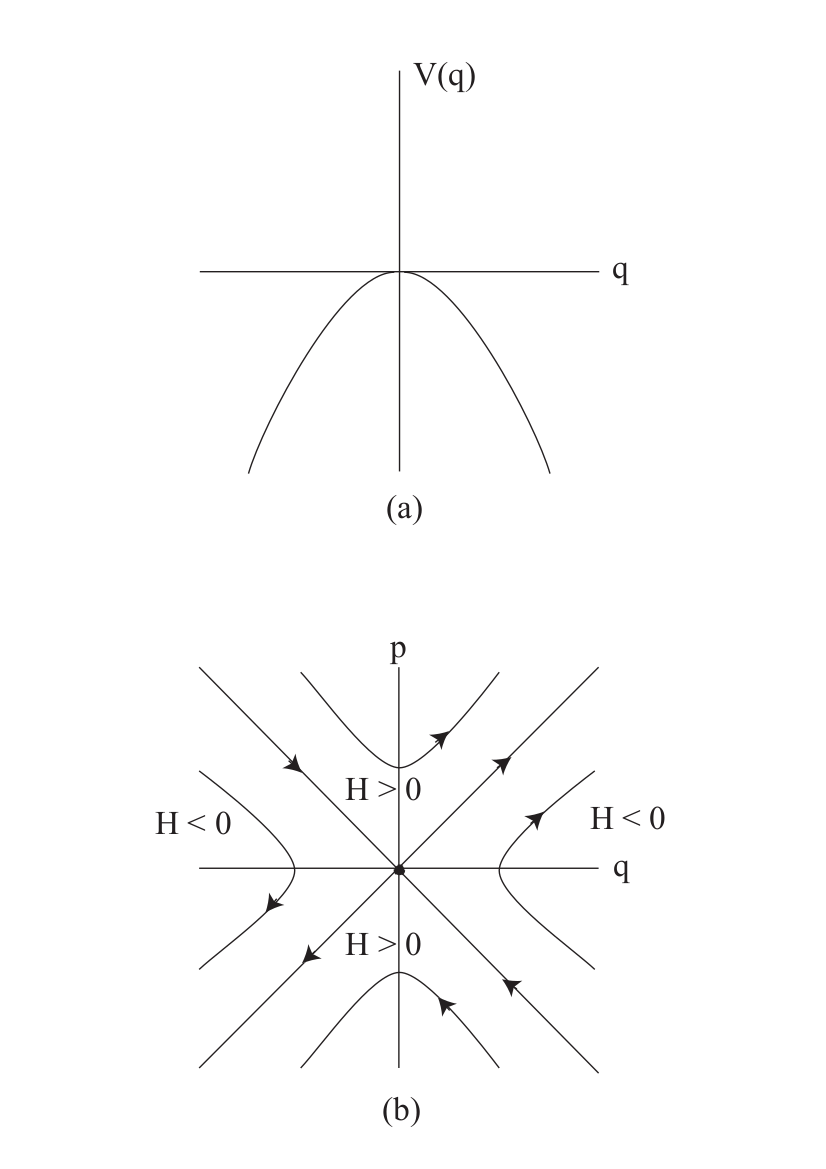
\includegraphics[width=6.0cm]{fig_1_dof_saddle.png}
\end{center}
\caption{a) The potential energy, $V(q) =-\frac{\lambda}{2} q^2$,  for a one DoF saddle. b)The phase space for the one DoF saddle.}
\label{fig:1 dof saddle}
\end{figure}

This is the archetypical one DoF Hamiltonian system modelling reaction dynamics associated with a saddle point. The only configuration space coordinate, $q$, is the reaction coordinate. 
In this simple system `'reaction'' corresponds to trajectories that change sign in $q$, which requires $H>0$ (as shown in Fig. \ref{fig:1 dof saddle} b)). Non-reacting trajectories have $H <0$. 

Now we discuss the NHIM, its stable and unstable manifolds, and their role in constructing the DS. All of these notions are `'trivial'' in this simple setting, but they will serve  to focus the ideas when we consider more DoF. 

For this case the NHIM  is the saddle point at the origin (a single `'point'' is a trivial example of a manifold). It only exists  on the $H=0$ energy surface (this is  very different when we go to two, and more, DoF) and its stable and unstable manifolds are the diagonal lines (also on the $H=0$ energy surface--the stable and unstable manifolds of a NHIM have the same energy as the NHIM). 

The non-isoenergetic DS can be taken as the line $q=0$. Clearly, it has the `'no-recrossing'' properties and all  reacting trajectories must cross this line. The DS at a fixed (positive) energy is  given by

\begin{equation}
\frac{\lambda}{2} p^2 = H = \mbox{constant},
\end{equation}

\noindent
or

\[
p =\pm \sqrt{\frac{2}{\lambda} H}.
\]


\noindent
So for a fixed energy $H > 0$ the DS consists of two distinct  {\em points}:  $p =+ \sqrt{\frac{2}{\lambda} H}$ (the dividing surface for forward reactions) and $p =- \sqrt{\frac{2}{\lambda} H}$ (the dividing surface for backward reactions).  These points are just the intersections of the reacting trajectories with $q=0$.







\end{document}


